\chapter{Применение ``CATIA-GDML geometry builder'' к CBM RICH}\label{sec:chapRICHgeom}

Значительная часть работы над ``Builder'' выполнялась при поддержке группы CBM RICH, поэтому самая сложная MC-модель, построенная с помощью ``Builder'', это CBM RICH. Модель была построена за несколько итераций, имеет достаточно сложную иерархию и характеризуется высокой степенью подробностей.
Геометрическая MC-модель детектора RICH эксперимента CBM имеет многоуровневую структуру, в основном обоснованную физической структурой сборки, но иногда и \todo бывает неочевидной и неестественной с целью повышения эффективности проведения частиц.
Для моделирования эксперимента в CBM используется пакет CbmRoot. Для того, чтобы GDML файлы, экспортированные из CATIA, корректно читались CbmRoot было написано дополнение, описанное в секции~\ref{sec:secFairModule}.

На момент написания данной работы инженерный проект не был завершён --- некоторые узлы были проработаны достаточно подробно и прошли несколько этапов уточнения, в которых модель менялась принципиально. В то же время некоторые узлы существуют лишь на концептуальном уровне. В первую очередь к ним относится форма и конструкция корпуса детектора, проектирование которой является относительно несложной задачей и может быль отложено на более поздний этап. Большая часть корпуса не оказывает влияния на эффективность детектора, т.к. лежит за пределами геометрического аксептанса, поэтому допускается моделирование физики детектора с упрощённой моделью корпуса, либо вообще без него.

%Кусок перенесён

В детекторе RICH можно выделить несколько подсистем --- фоточувствительная камера, магнитный экран вокруг камеры, зеркала, система опор зеркал, часть ионопровода в RICH, корпус детектора. Рассмотрим реализацию каждой подсистемы в MC-модели, построенной с помощью ``CATIA-GDML geometry builder''.

% ==============================================================================================
% ==============================================================================================
% ==============================================================================================

\section{Фокусирующая система --- сферические зеркала}\label{sec:secRICHgeoMirror}

%Кусок перенесён

Далее рассматривается только одно, верхнее зеркало. Всё описание распространяется и на симметричное нижнее зеркало.

%Основная задача зеркал --- отвести черенковские фотоны в область, где они могут быть зарегистрированы фоточувствительной камерой, которую невозможно расположить напрямую на пути этих фотонов, т.е. в геометрической аксептансе. Это сделает работу последующих детекторов невозможным из-за вторичных частиц.
Основная задача зеркал --- сфокусировать черенковский свет на фоточувствительную камеру. Также присутствет возможность, изменяя угол наклона зеркал, выбирать расположение камеры.

Вообще есть целое направление, в котором люди занимаются тем, что оценивают и обычно стараются минимизировать material budget.

Для того, чтобы фокусировать фотоны на камеру, расположенную за пределами аксептанса, необходимо, чтобы центр сферической поверхности располагался над осью пучка, а сами зеркала полностью покрывали акспетанс. Есть как минимум два варианта геометрии зеркал. В первом зеркало выполняется симметричным относительно горизонтальной плоскости и поворачивается вокруг оси X. При этом возникает зазор между двумя зеркалами, расширяющийся к краям (см. \figref{}), но все зеркала составляются из сегментов двух типов. Более оптимальный способ --- выбрать правильную долю сферы так, чтобы зеркала стыковались без зазора. При этом зеркало получается несимметричным, а следовательно необходимо 4 типа сегментов. Данный вопрос также затрагивается в \ref{sec:secMirrorsEvolution}

% Кусок перенесён

В связи с такими-то причинами
, корректируя отклонения от правильного положения, связанные с перемещениями точек механической опоры, находящейся в напряжённо-деформированном состоянии под собственным весом и весом зеркал. Также возможны перемещения в связи с термическим расширением рамы при изменении параметров окружающей среды в экспериментальном зале.

Коллаборациями LHCb и COMPASS разработаны методы \todo, позволяющие выполнять...
Для анализа в моделировании необходимо обеспечить возможность поворота отдельных сегментов зеркал вокруг заданных осей. В связи с этим была построена версия MC-модели, отличающаяся структурой объёмов и обеспечивающая возможность поворота отдельных сегментов зеркал вокруг заданных осей. Эта модель обсуждается в \ref{sec:secRICHgeoMirrorMis}.

\subsection{MC-геометрия фокусирующей системы с возможностью задания индивидуальных отклонений}\label{sec:secRICHgeoMirrorMis}

Для отладки методов калибровки положения зеркал необходимо выполнять моделирование с геометрией, имеющей отклонения сегментов зеркал, заданные определённым образом. Техника \todo CLAM разработана с расчётом на то что отклонение каждого сегмента может быть получено в результате двух вращений. Если для каждого сегмента зеркала ввести фиксированный центр и локальную систему координат с осями $\overrightarrow{n}$, $\overrightarrow{\tau}$ и $\overrightarrow{b}$, то вращение должно осуществляться последовательно вокруг \todo.

Для того, чтобы это было возможно в разработанной MC-модели CBM RICH потребовалось ввести два промежуточных уровня вложенности --- один для каждого типа зеркал и ещё один для каждого сегмента. Первый промежуточный уровень вложенности переносит центр сегмента в начало координат. Второй обеспечивает вращение вокруг оси \todo. При позиционировании в газ вводится отклонение вокруг второй оси \todo.

\todo \textbf{уточнить}

Одна из задач, которую приходится решать с описываемой геометрией --- выполнять многократно моделирование прохождения частиц с разными значениями отклонения сегментов зеркал. Это означает, что пользователь должен иметь возможность легко модифицировать геометрию. По этой причине значения отклонений каждго сегмента зеркала были вынесены в качестве параметров модели, что выглядит как список из 160 параметров в <define> секции GDML файла. Имя каждого параметра построено по правилу ``misalign\textunderscore AXIS\textunderscore A\textunderscore B'', где AXIS --- осьвращения --- либо ``x'', либо ``y'', $A \in [0,7]$ --- номер сегмента вдоль вертикального направления, а $B \in [0,9]$ --- номер сегмента вдоль горизонтального направления.

\todo \textbf{картинка с нумерации сегментов зеркал}

В итоге получается две модели RICH --- одна для общего пользования с идеально позиционированными зеркалами и вторая отдельно для отладки методов коррекции положения зеркал. Для того, чтобы не \todo плодить сущности без необходимости оба зеркала смоделированы в одной CATIA сборке, а разделение на два GDML файла выполняется путём комментирования некоторых частей одного GDML файла, экспортируемого из CATIA. Использование геометрии с индивидуальным отклонениями зеркал для моделирования в общей установке CBM не рационально, т.к. в такой геометрии больше объёмов. Кроме того, в геометрии с отклонениями зеркал по запросу пользователя были выключены некоторые подробности (такие как, например, каркас детектора и опоры зеркал), т.к. они не оказывают никакого влияния на исследование CLAM, но замедляют моделирование.

% ==============================================================================================
% ==============================================================================================
% ==============================================================================================

\section{Магнитный экран вокруг камеры}\label{sec:secCameraShield}

% Кусок перенесён

Т.к. рассматривалось два варианта форм фоточувствительной камеры --- четыре плоскости и два цилиндра --- потребовалось прорабатывать два варианта формы магнитного экрана. На \figref{fig:ShieldingBox} показан чертёж первого рассчитанного магнитного экрана для плоского варианта камеры, а на \figref{fig:ShieldingBoxMC} --- первая версия магнитного экрана в CbmRoot.

% Перенесено из RICHgeom
\begin{figure}[H]
\centering
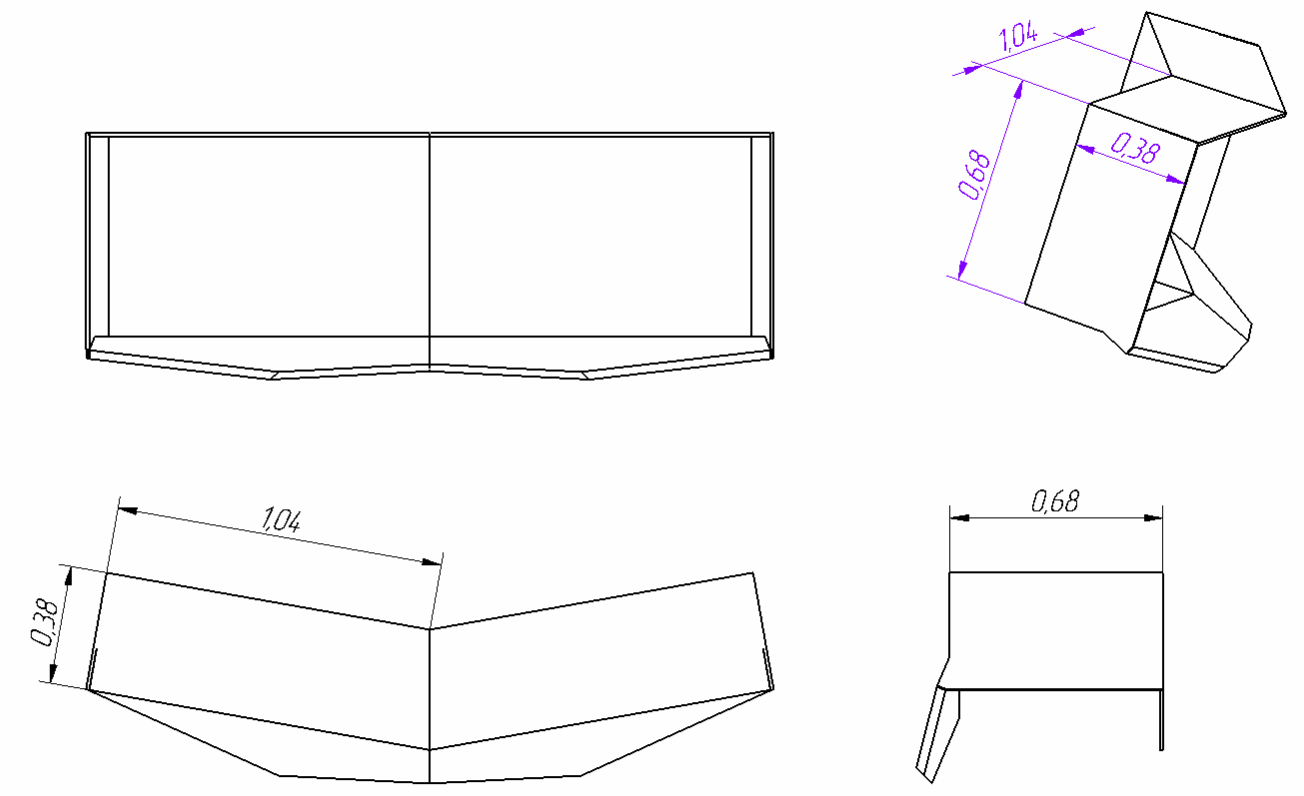
\includegraphics[width=0.7\textwidth]{pictures/First_shielding_box_1.png}
\caption{Первый эскизный проект магнитного экрана.}
\label{fig:ShieldingBox}
\end{figure}

% Перенесено из RICHgeom
\begin{figure}[H]
\begin{minipage}[b]{0.495\textwidth}
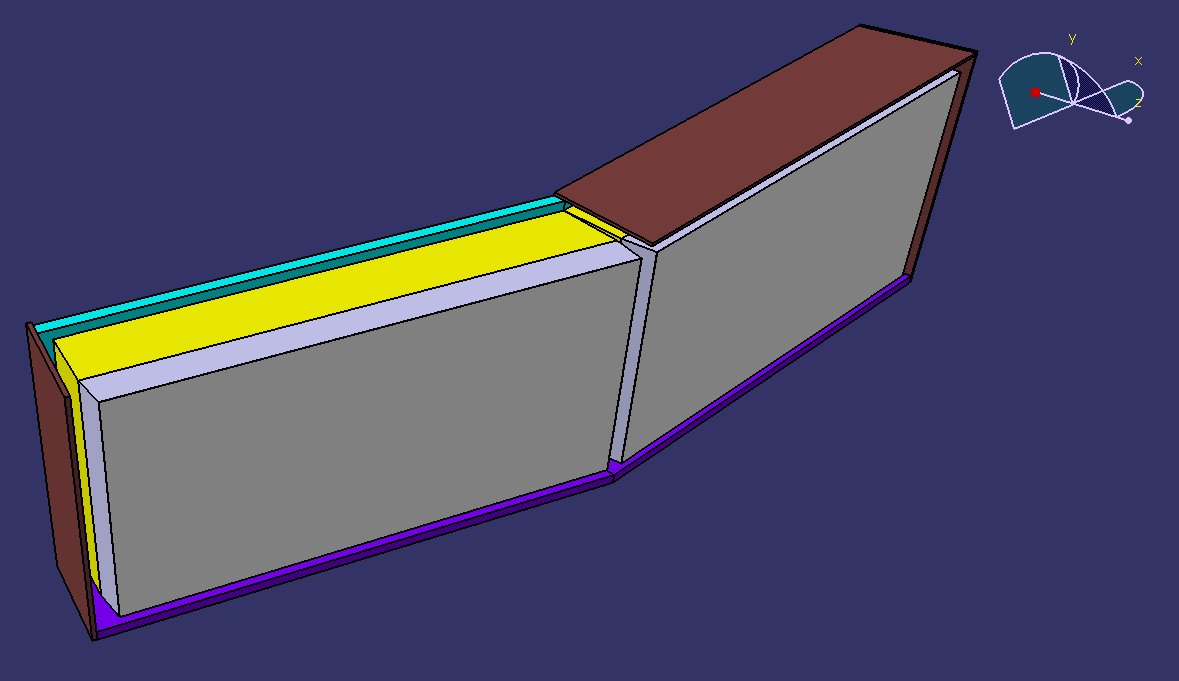
\includegraphics[width=1.0\textwidth]{pictures/ShieldingBox_MC.png}
\end{minipage}
\hspace{0.01\textwidth}
\begin{minipage}[b]{0.495\textwidth}
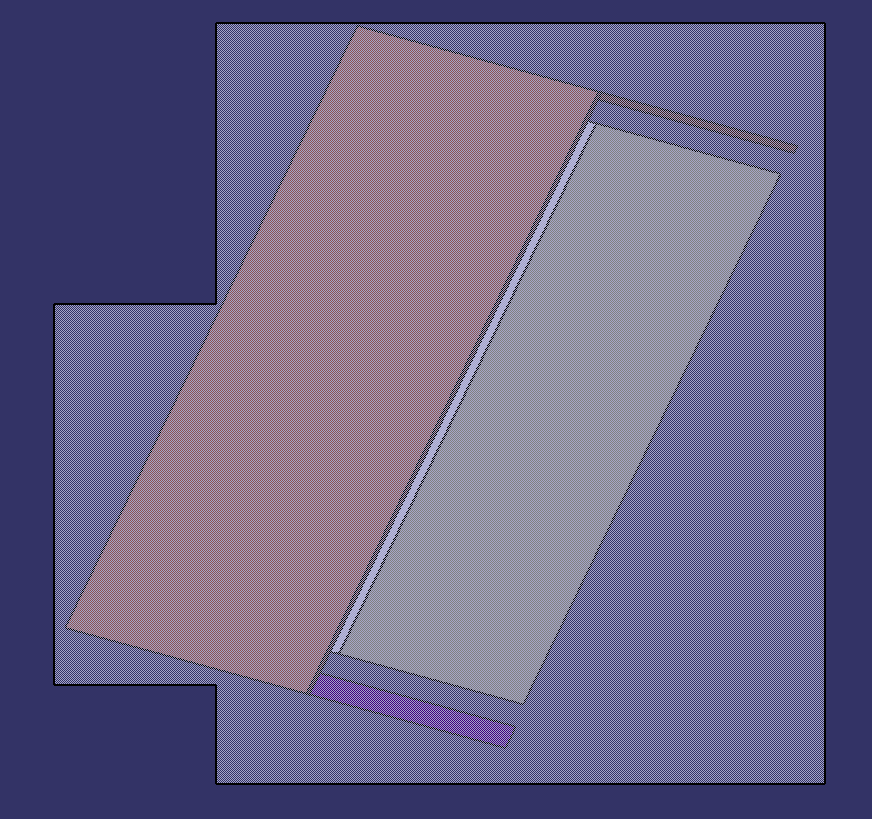
\includegraphics[width=0.7\textwidth]{pictures/ShieldingBox_MC2.png}
\end{minipage}
\caption{Первая версия магнитного экрана в CbmRoot. Серым цветом показаны МА~ФЭУ, жёлтым --- электроника.}
\label{fig:ShieldingBoxMC}
\end{figure}

% Перенесено из RICHgeom
На момент написания данной работы проект магнитного экрана не был завершён, однако было выполнено эскизное проектирование и моделирование распределения магнитного поля в пакете OPERA (TOSKA). Было определено, что магнитный экран должен иметь нижнюю и заднюю (ближную к магниту) стенку толщиной 30~мм, а остальные --- толщиной 10~мм. Одной из проблем при проектировании магнитного экрана является задача минимизации массы; т.к. экран должен быть выполнен из материала с высоким коэффициентом магнитной проницаемости, лёгкие металлы типа алюминия не подходят. Масса каждого из двух экранов получилась равна 850~кг. В экране присутствуют отверстия необходимые для отвода кабелей и для обеспечения охлаждения.

% ==============================================================================================
% ==============================================================================================
% ==============================================================================================

\section{Фоточувствительная камера}\label{sec:secRICHgeoCamera}

Планируется, что фоточувствительная камера CBM RICH будет составлена из модулей, содержащих 2$\times$3 МА~ФЭУ Hamamatsu H12700, см. \figref{fig:H12700drawing}. Один такой МА~ФЭУ имеет габариты 52$\times$52~мм$^2$, между МА~ФЭУ оставляется зазор 1~мм для запаса по точности, таким образом размер модуля составляет 158мм$\times$105мм.

\begin{figure}[H]
\centering
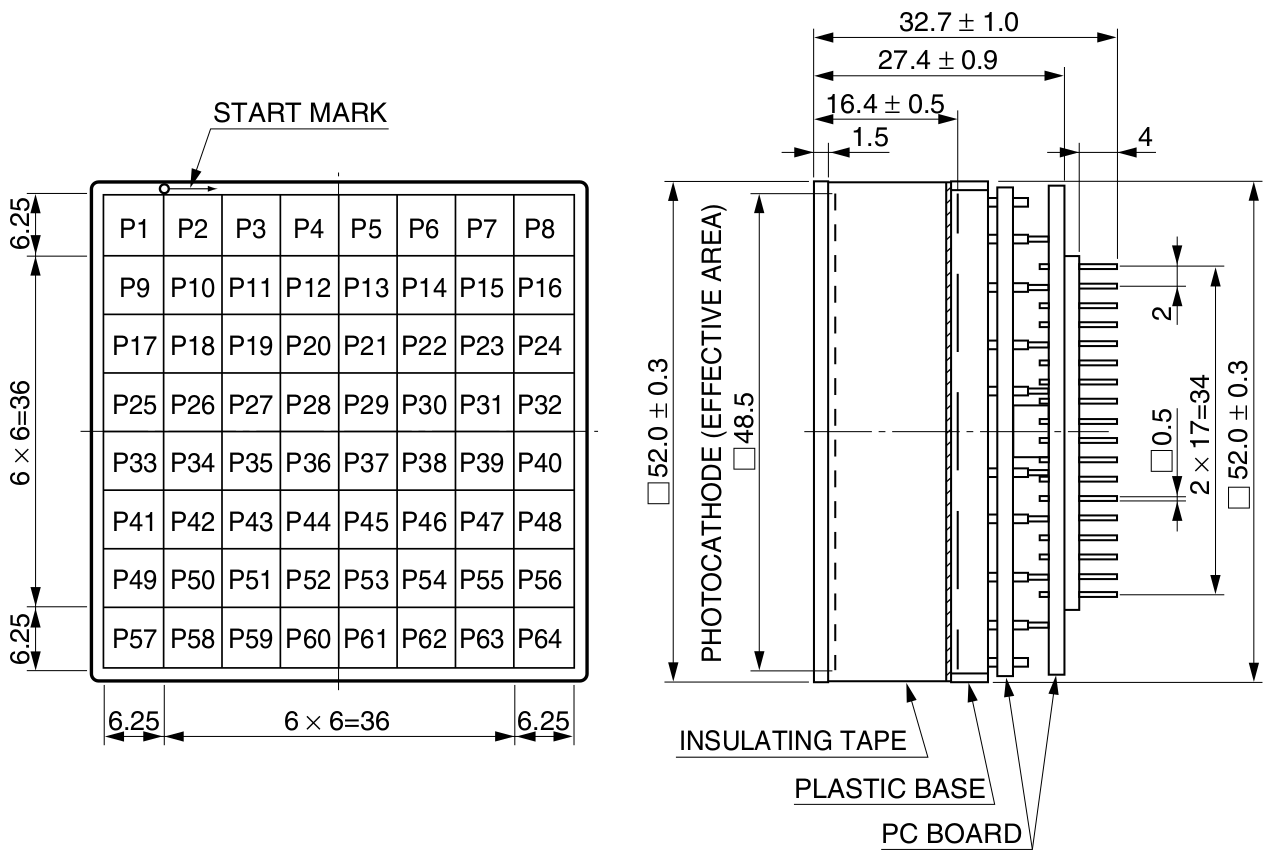
\includegraphics[width=0.7\textwidth]{pictures/H12700_drawing.png}
\caption{Чертёж МА~ФЭУ H12700 из документации.}
\label{fig:H12700drawing}
\end{figure}

В момент написания данной работы ведётся работа по проектированию модуля, разработке программ для FPGA, но имеются изготовленный прототип. Помимо МА~ФЭУ в модуль входят 12~плат передней электроники DIRICH, одна плата, обеспечивающая питание, и одна плата концентрации данных. В основе модуля лежит плата-адаптер, к которой с одной стороны подсоединяются МА~ФЭУ, а с другой --- все платы. CAD-модель и MC-модель модуля показаны на \figref{fig:geoMCmodule}.

\begin{figure}[H]
\begin{minipage}[b]{0.495\textwidth}
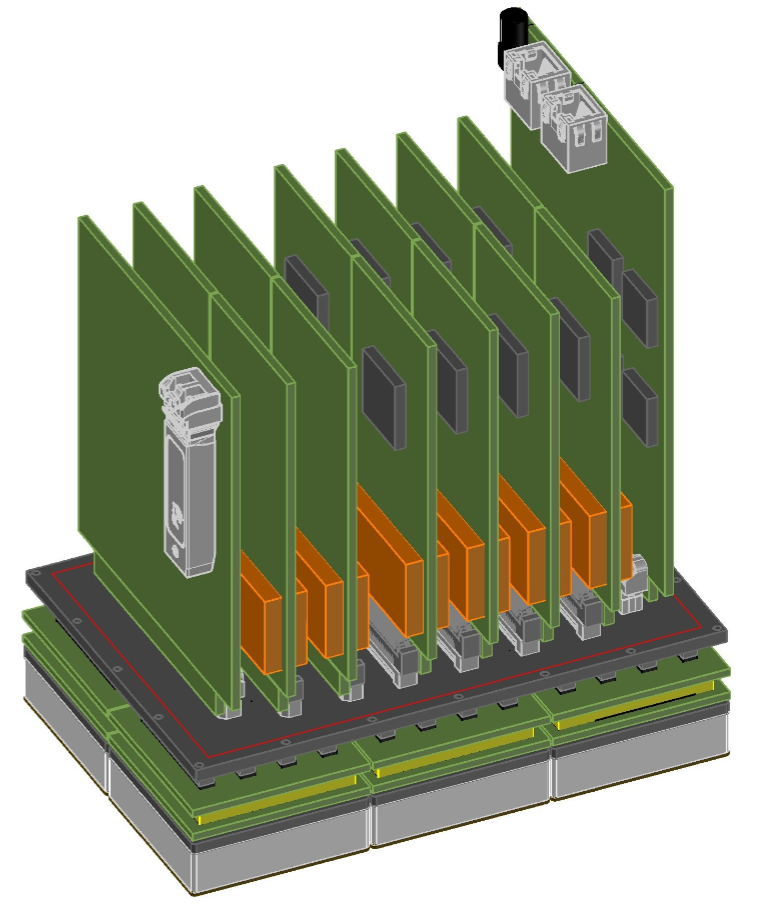
\includegraphics[width=1.0\textwidth]{pictures/PMTmoduleCAD.png}
\end{minipage}
\hspace{0.01\textwidth}
\begin{minipage}[b]{0.495\textwidth}
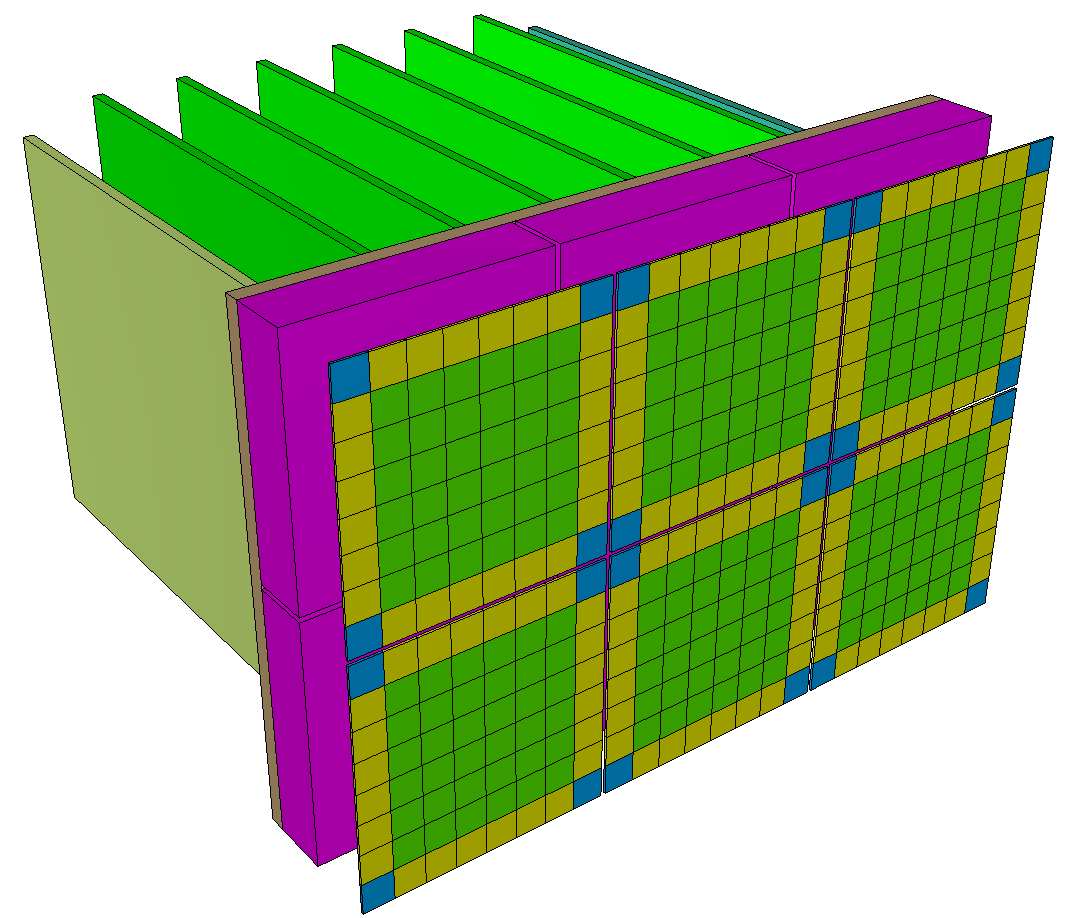
\includegraphics[width=1.0\textwidth]{pictures/Module_1_cut.png}
\end{minipage}
\caption{CAD-модель (слева) и MC-модель (справа) модуля фоточувствительной камеры CBM RICH.}
\label{fig:geoMCmodule}
\end{figure}

Иерархия объёмов, моделирующих модуль фоточувствительной камеры CBM RICH приведена на \figref{fig:Module_geoStructure}.

\begin{figure}[H]
\centering
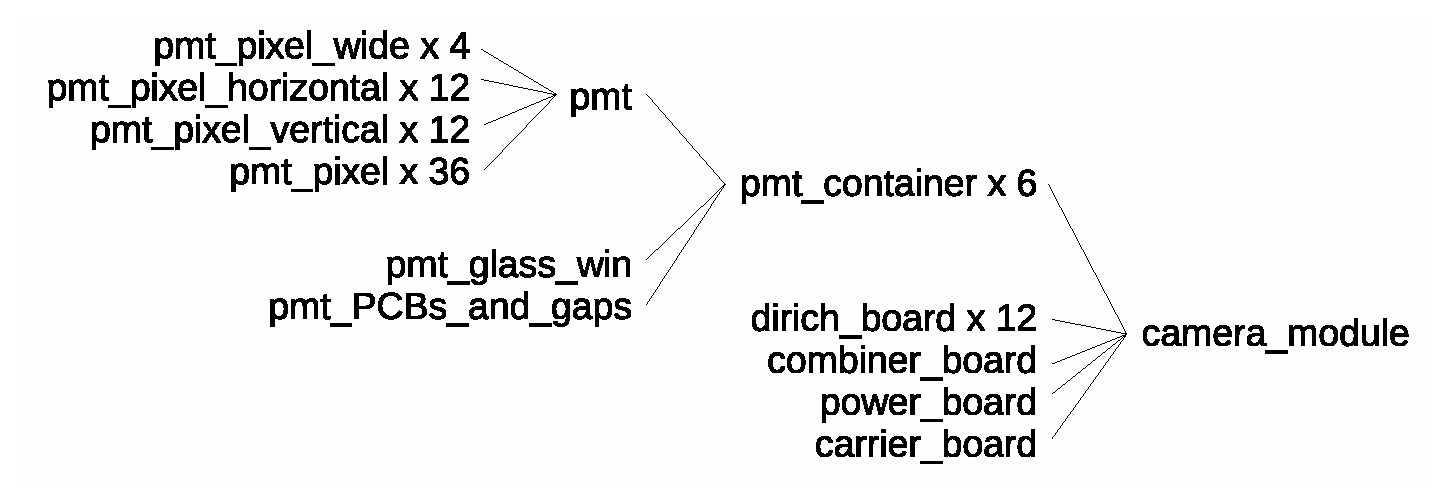
\includegraphics[width=0.7\textwidth]{pictures/Module_geoStructure.eps}
\caption{Иерархия объёмов, моделирующих модуль фоточувствительной камеры CBM RICH.}
\label{fig:Module_geoStructure}
\end{figure}

%Пиксели
%№№ 2-7, 58-63, 9, 17,..., 49, 16, 24,..., 56
МА~ФЭУ моделируется до уровня пикселей. Это позволяет максимально приблизить моделирование прохождения частиц в CbmRoot и обработку реальных данных. В соответствии с документацией, у МА~ФЭУ H12700 пиксели имеют разные размеры (см. \figref{fig:H12700drawing}): угловые пиксели (№№ 1, 8, 57, 64) 6.25мм$\times$6.25мм, пиксели по краям, кроме угловых, --- 6.25мм$\times$6мм, остальные, центральные пиксели --- 6мм$\times$6мм. Для того, чтобы представить три типа пикселей в MC-модели, необходимо три отдельных объёма, имеющих разную форму. Чтобы сделать модель максимально понятной и гибкой принято решение отделить пиксели из крайних горизонтальных рядов от пикселей из крайних вертикальных рядов и моделировать их с помощью двух разных объёмов размером 6мм$\times$6.25мм и 6.25мм$\times$6мм соответственно. Это позволит позиционировать все пиксели без поворотов.

Таким образом вводится три объёма: \volumename{pmt\textunderscore pixel\textunderscore wide} для угловых пикселей, \volumename{pmt\textunderscore pixel\textunderscore horizontal} для пикселей в крайних горизонтальных рядах, \volumename{pmt\textunderscore pixel\textunderscore vertical} для пикселей в крайних вертикальных рядах и \volumename{pmt\textunderscore pixel} для всех остальных пикселей, расположенных в центральной зоне. Все 4 объёма имеют форму примитива box с толщиной вдоль оси Z, равной 0.5мм, материал CsI, который в данный момент используется в моделировании как активный материал для фоточувствительных элементов. Толщина выбрана произвольно, она не имеет значения, т.к. из-за того, что материал объёма активный, т.е. объём объявлен чувствительным, система проведения частиц будет вырабатывать сигнал о пересечении треком границы объёма и передавать управление методу \methodname{ProcessHits} класса детектора \classname{CbmRich}. В реализации этого метода вырабатывается Point, причём физика не оказывает никакого влияния. Даже если толщина объёма слишком маленькая, чтобы произошло какое-либо взаимодействие, флаг активности обязывает систему вызвать \methodname{ProcessHits}.

Объём \volumename{pmt} соответствует части МА~ФЭУ, включающей в себя фотокатод (пиксели) и динодную систему, и имеет толщину $16.4-1.5=14.9$мм. Входное стеклянное окно МА~ФЭУ моделируется отдельным объёмом \volumename{pmt\textunderscore glass\textunderscore win}, имеющим толщину 1.5мм. Пространство за динодной системой, включающее в себя печатные платы и ножки в воздушном пространстве, моделируется объёмом \volumename{pmt\textunderscore PCBs\textunderscore and\textunderscore gaps}. Все части МА~ФЭУ, моделируемые перечисленными объёмами, вставляются в контейнер \volumename{pmt\textunderscore container}.

Платы передней электроники, питания, концентрации данных и палата-адаптер моделируются объёмами, имеющими форму box и одинаковый материал, --- \volumename{dirih\textunderscore board}, \volumename{power\textunderscore board}, \volumename{combiner\textunderscore board}, и \volumename{carrier\textunderscore board} соответственно. Объём \volumename{camera\textunderscore module} выполняет роль контейнера, в который помещаются МА~ФЭУ и платы. Далее составляется вертикальный массив из \todo 7 модулей, называемый \volumename{camera\textunderscore strip}.

В процессе разработки детектора сначала рассматривался вариант фоточувствительной камеры, состоящей из 4 плоскостей, расположенных симметрично относительно горизонтальной и вертикальной плоскостей, проходящих через ось пучка. Исследовались разные варианты комбинаций размера, поворотов и положения четверти с целью нахождения оптимальных значений с точки зрения эффективность всего детектора. Одна итерации такой оптимизации заключается в запуске полного моделирования и анализа и является достаточно время-затратной процедурой.

В настоящее время прорабатывается вариант, в котором верхняя и нижняя половины фоточувствительной камеры составлены из сегментов шириной в один модуль и аппроксимирующих поверхность цилиндра. Радиус 1650~мм, поворот $\SI{18}{\degree}$ вокруг оси X и положение цилиндра также получены в результате оптимизации.

\begin{figure}[H]
\begin{minipage}[b]{0.495\textwidth}
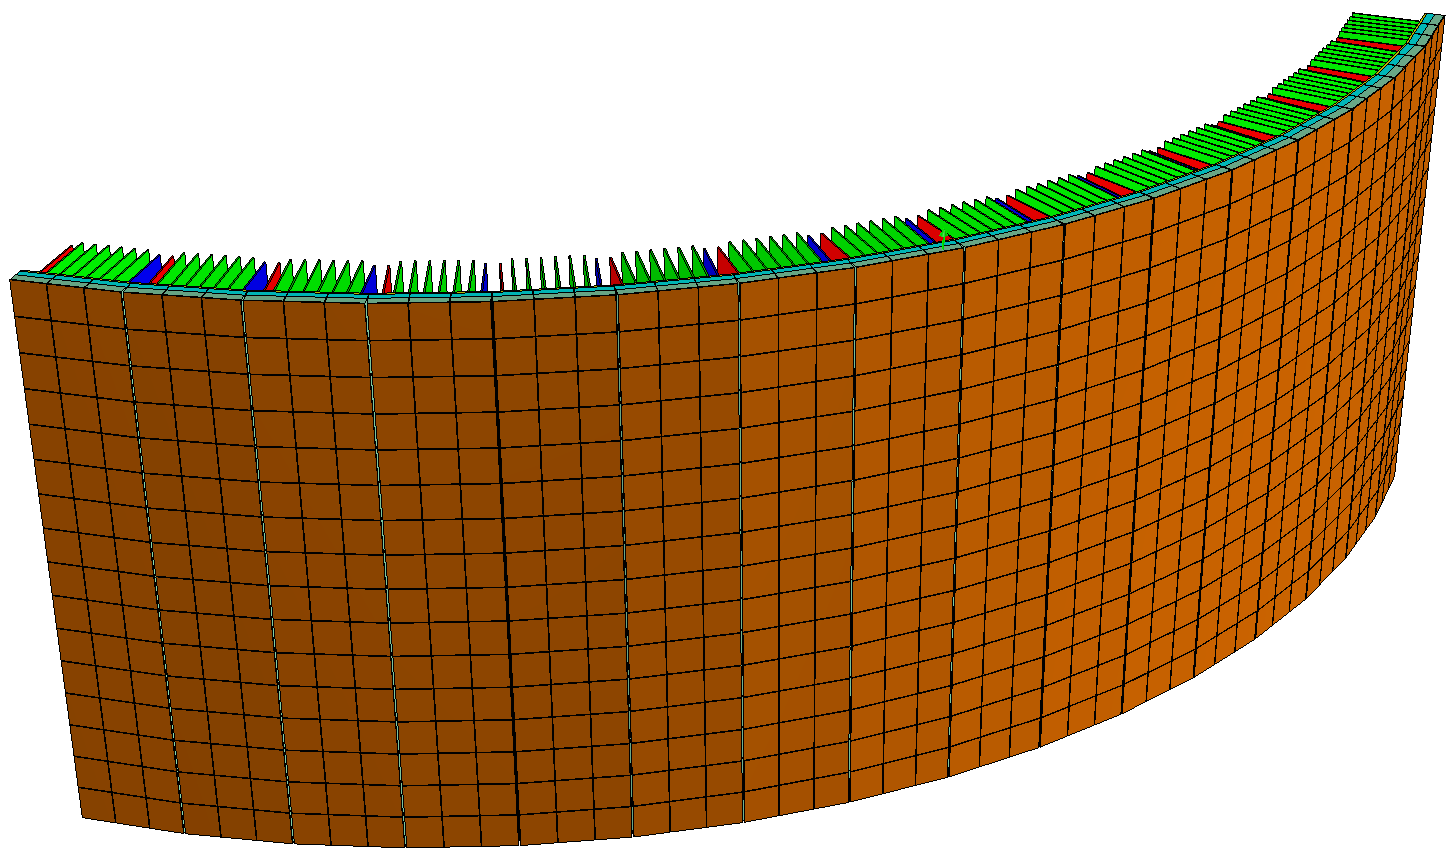
\includegraphics[width=1.0\textwidth]{pictures/Camera_pmts.png}
\end{minipage}
\hspace{0.01\textwidth}
\begin{minipage}[b]{0.495\textwidth}
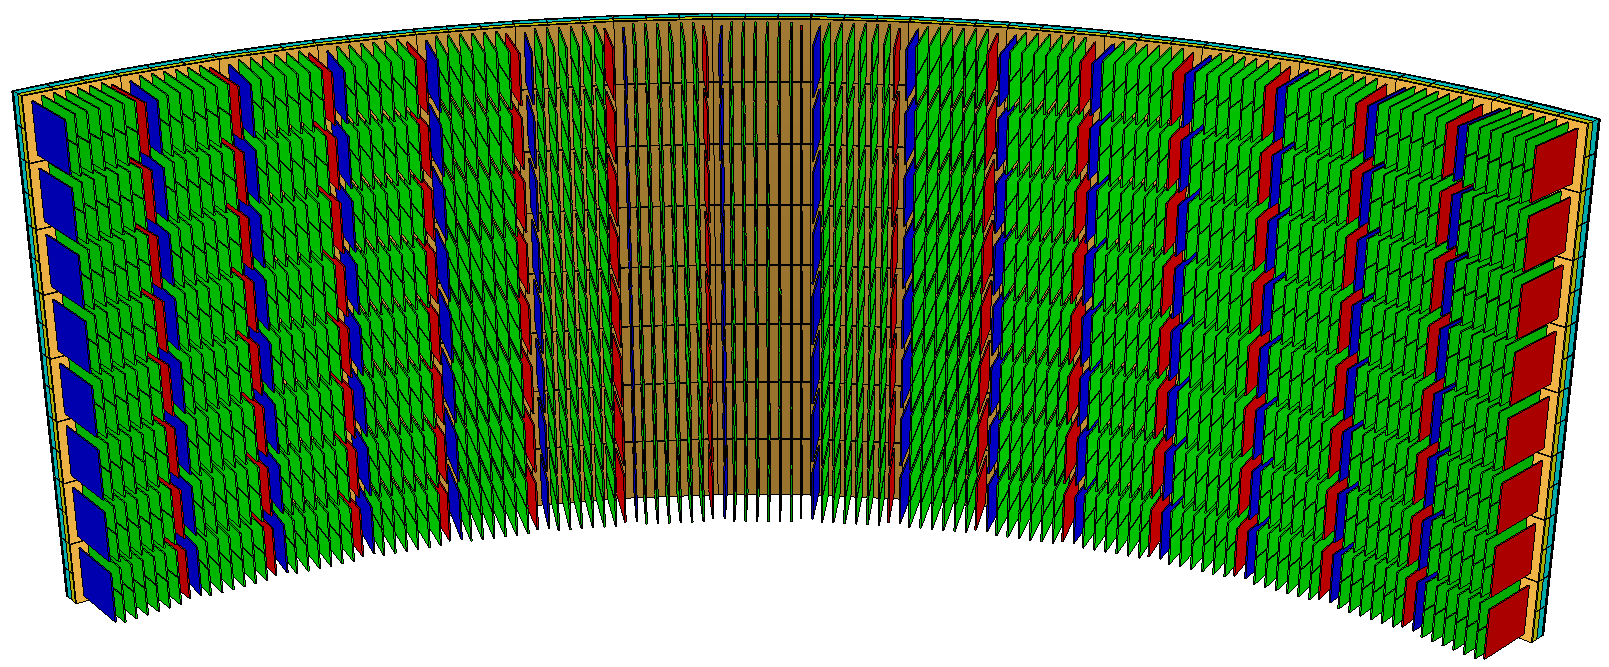
\includegraphics[width=1.0\textwidth]{pictures/Camera_back.png}
\end{minipage}
\caption{MC-модель фоточувствительной камеры CBM RICH. На рисунке показаны платы электроники, но не показаны отдельные пиксели МА~ФЭУ.}
\label{fig:geoMCcamera}
\end{figure}

% ==============================================================================================
% ==============================================================================================
% ==============================================================================================

\section{MC-геометрия механических конструкций RICH}\label{sec:secRICHgeoMech}

Различные механические конструкции не участвуют в физической части функционирования детектора, а лишь выполняют функцию опоры и, в случае CBM RICH, создают герметичный контейнер для газового радиатора. В CBM RICH можно выделить следующие крупные пассивные составляющие --- корпус детектора, опоры зеркал, несущая конструкция и магнитный экран фоточувствительных камер. Несмотря на то, что такие конструкции являются пассивными, они всё же оказывают влияние на эффективность детектора, т.к. частицы взаимодействуют с их материалом и в результате могут изменить направление и импульс, поглотиться или произвести вторичные.

Чтобы оценить влияние материала механических конструкций на функционирование детектора необходимо максимально точно смоделировать количество материала в аксептансе. Применение ``CATIA-GDML geometry builder'' сильно облегчает процесс моделирования пассивного материала, т.к. стандартными средствами CATIA можно измерить объём детали сложной формы, чтобы затем использовать это значение для расчёта упрощённой детали.

Приведём решение типовой задачи. Требуется заменить сложный профиль прямоугольным кольцом с совпадающими внешними размерами. Наиболее оптимально моделировать балку с таким профилем с помощью двух вложенных объёмов, имеющих форму box. Более крупный объём выполнен из металла, а дочерний --- из материала окружающей среды (в случае CBM RICH --- газ-радиатор).

\begin{figure}[H]
\begin{minipage}[b]{0.495\textwidth}
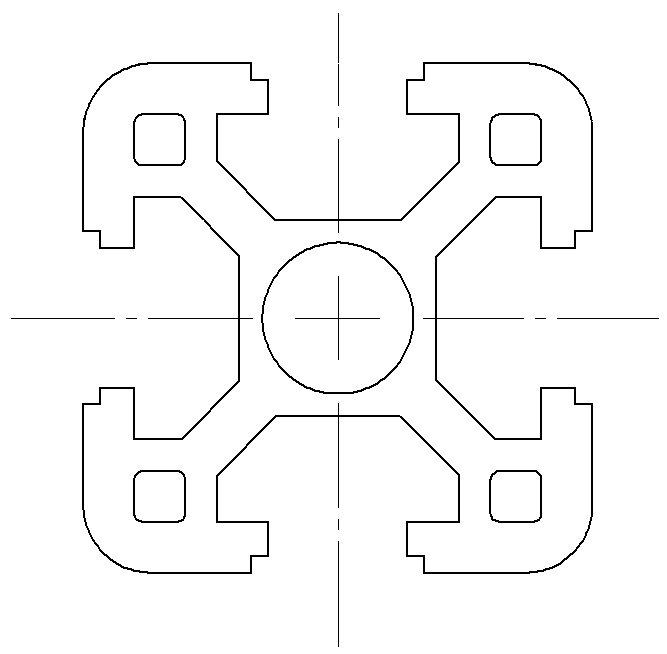
\includegraphics[width=0.8\textwidth]{pictures/Complex_profile.png}
\end{minipage}
\hspace{0.01\textwidth}
\begin{minipage}[b]{0.495\textwidth}
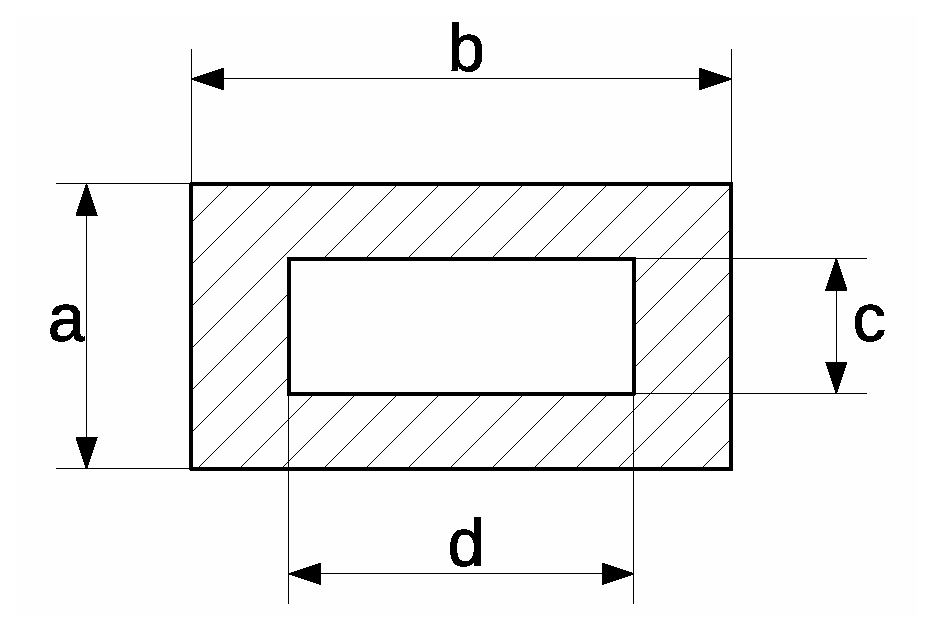
\includegraphics[width=1.0\textwidth]{pictures/Material_budget.eps}
\end{minipage}
\caption{Исходный профиль в CAD-модели (слева) и итоговый профиль в MC-модели.}
\label{fig:geoProfiles}
\end{figure}

Площадь исходного профиля $S_{CAD}$ измеряется стандартной функцией CATIA~v5. Задача заключается в том, чтобы определить размеры $a, b, c, d$ в MC-модели такие, что площадь обоих профилей совпадает, т.е. $S_{CAD} = S_{MC}$. Пользователь может выбрать внешние размеры $a$ и $b$, например так, чтобы они совпадали с габаритами исходного профиля. Очевидно, $S_{MC} = ab - cd$. Пусть $c = ka$ и $d = kb$. Тогда $S_{CAD} = S_{MC} = ab - ka \cdot kb = ab(1 - k^2)$. Отсюда $1 - k^2 = \frac{S_{CAD}}{ab}$ и $k = \sqrt{1 - \frac{S_{CAD}}{ab}}$. Отсюда вычисляются $c$ и $d$.

Механические конструкции RICH были построены с применением описанной методики. На \figref{fig:geoMainframe} приведена модель каркаса детектора в MC-формате в CATIA. Каждая балка моделируется отдельным объёмом, полость внутри балки моделируется с помощью дочернего объёма из материала окружающей среды, в данном случае --- газа радиатора. Одинаковые балки моделируются одним объёмом, который многократно вставляется в контейнер. Для того чтобы упростить позиционирование каркаса в материнском объёме, вся конструкция была собрана в двух объёмах типа Assembly (см. \figref{fig:geoMainframe1and2}).

\begin{figure}[H]
\begin{minipage}[b]{0.495\textwidth}
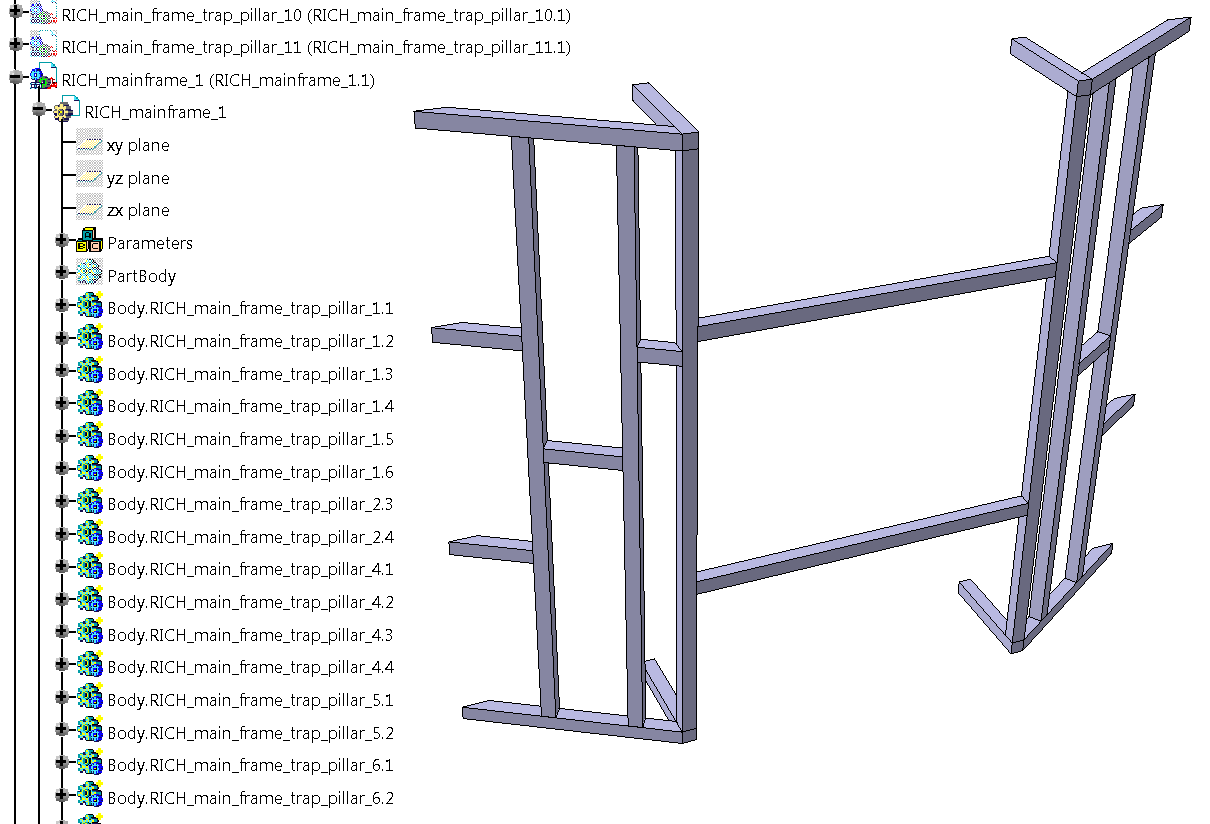
\includegraphics[width=0.8\textwidth]{pictures/Mainframe_1.png}
\end{minipage}
\hspace{0.01\textwidth}
\begin{minipage}[b]{0.495\textwidth}
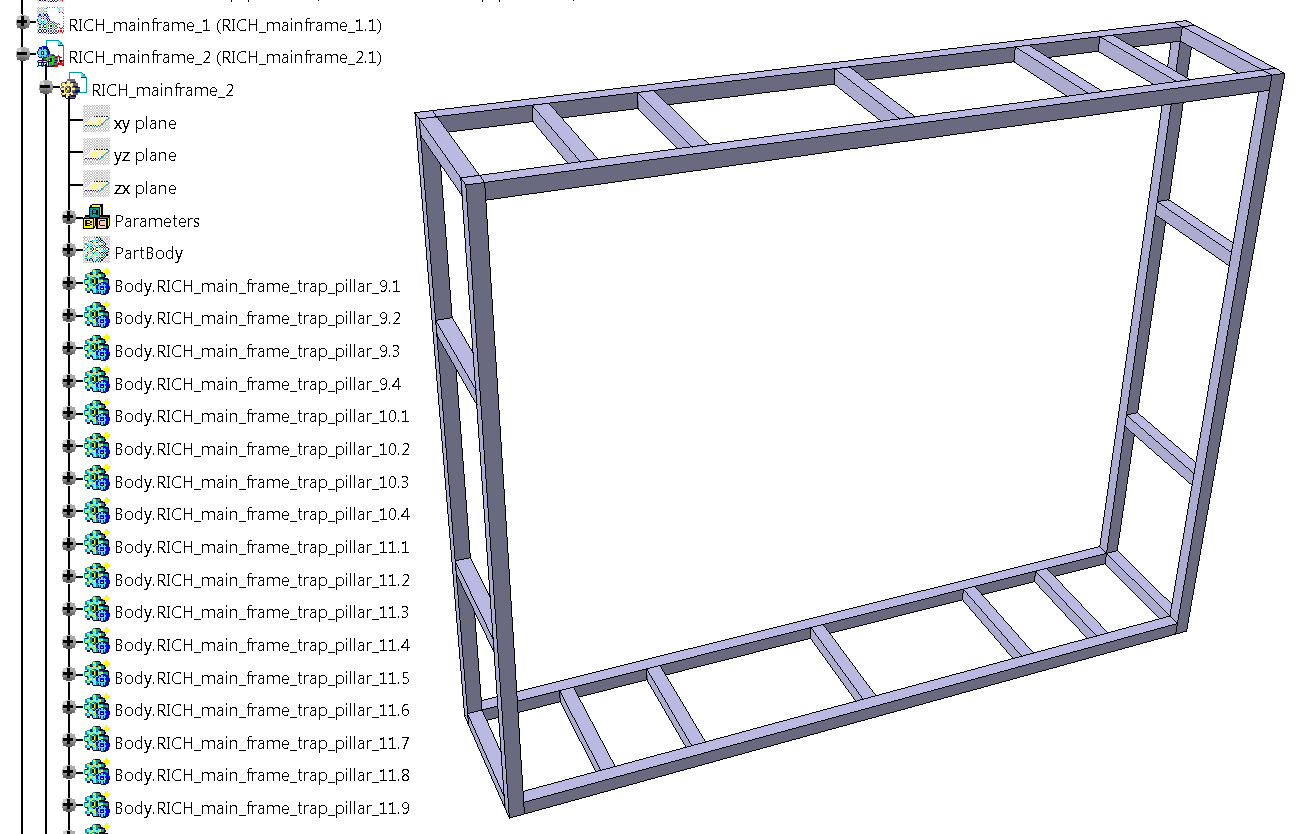
\includegraphics[width=1.0\textwidth]{pictures/Mainframe_2.png}
\end{minipage}
\caption{MC-модель двух частей каркаса детектора в CATIA.}
\label{fig:geoMainframe1and2}
\end{figure}

\begin{figure}[H]
\centering
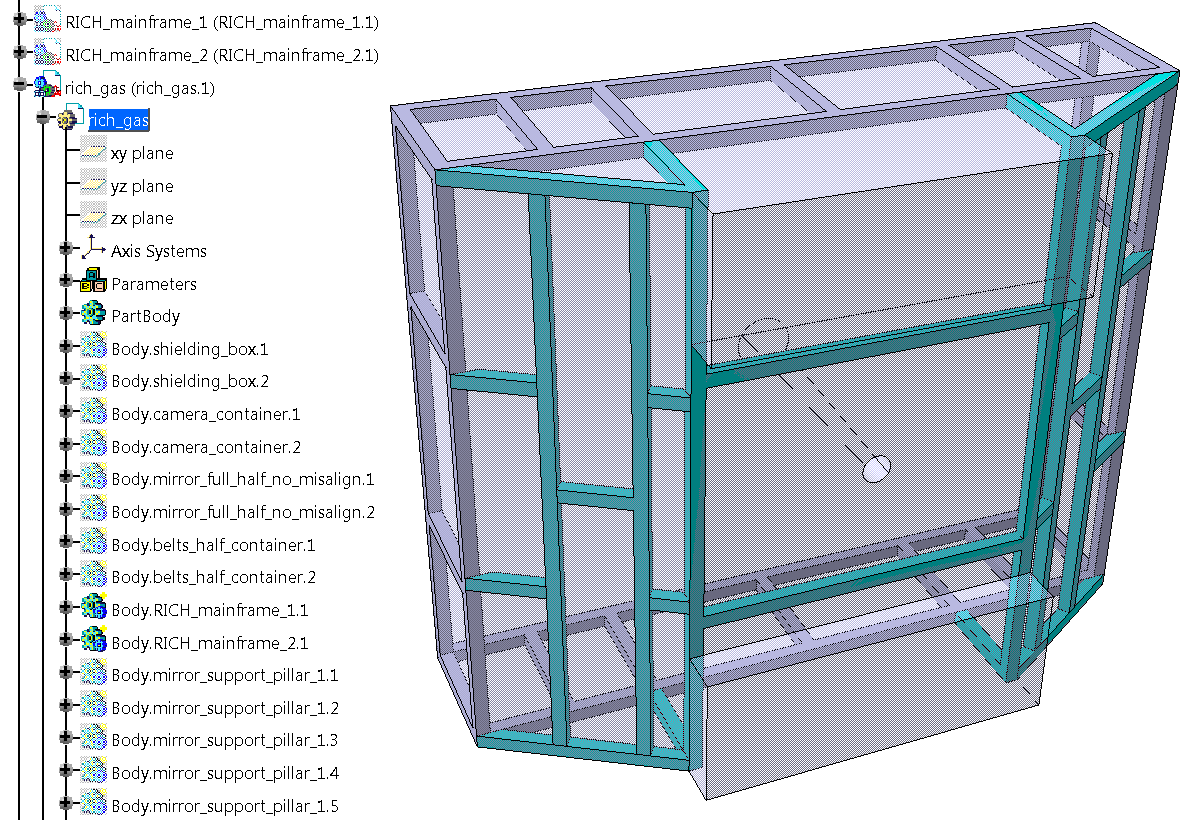
\includegraphics[width=0.7\textwidth]{pictures/Mainframe.png}
\caption{MC-модель каркаса детектора в материнском объёме в CATIA.}
\label{fig:geoMainframe}
\end{figure}

% ==============================================================================================
% ==============================================================================================
% ==============================================================================================

\section{История развития MC-модели CBM RICH.}\label{sec:secRICHgeoHistory}

На протяжении нескольких лет работы над проектированием детектора было создано несколько версий MC-геометрии CBM RICH. В основном, каждая следующая версия либо уточняла предыдущую, либо включала в себя обновления каких-то подсистем. Стоит отметить несколько устаревших на данный момент версий, в которых были внесены значительные изменения в соответствии с обновляющимся проектом детектора.

\subsection{Модель с примитивным фотодетектором.}

Первоначально рассматривался вариант, в котором фоточувствительная камера была составлена из четырёх плоскостей, расположенных симметрично относительно горизонтальной и вертикальной плоскостей. Начиная с самых ранних версий в модели RICH в CbmRoot камера была выполнена с помощью тонких пластин из активного материала, причём размер этих пластин был выбран так, чтобы полностью покрывать аксептанс, никак не соотносясь с реальными возможностями. На \figref{fig:PrimitivePhotodetector} показана часть модели CBM RICH с примитивным фотодетектором.

\begin{figure}[H]
\centering
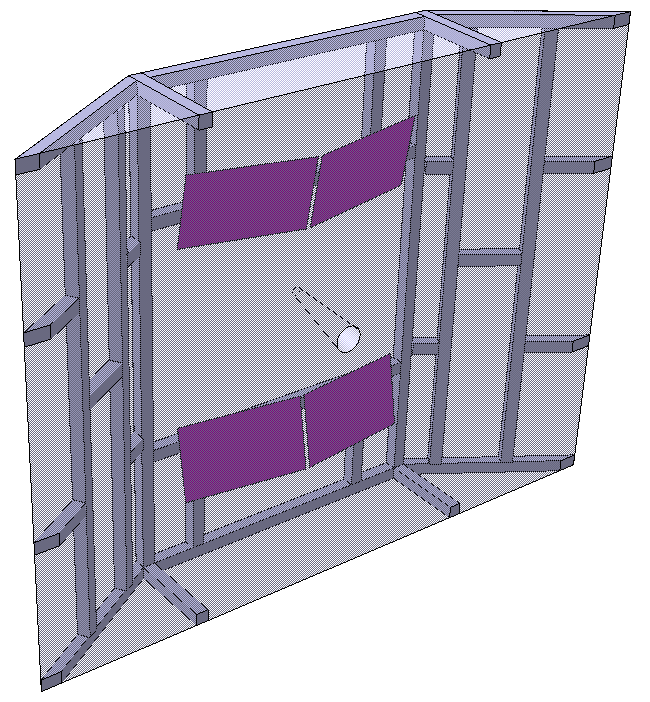
\includegraphics[width=0.6\textwidth]{pictures/PrimitivePhotodetector.png}
\caption{Часть одной из наиболее ранних MC-моделей CBM RICH, в которой фотодетектор был представлен тонкими чувствительными боксами.}
\label{fig:PrimitivePhotodetector}
\end{figure}

\subsection{Модель без магнитного экрана.}

Длительное время MC-модель CBM RICH не имела магнитного экрана, см. \figref{fig:MCgeoMirrorsEvolution}(слева). По этой причине не было необходимости создавать дополнительное пространство для выступающей части, что делало форму материнского объёма значительно более простой.

\subsection{Модель с промежуточным объёмом для магнитного экрана.}

В первой версии MC-модели с магнитным экраном был введён дополнительный промежуточный объём, позиционированный параллельно системе координат объёма радиатора. В него были на одном уровне помещены пластины, представляющие стенки экрана и ещё два контейнера --- с МА~ФЭУ и электроникой (см. \figref{fig:ShieldingBoxMC}). На момент написания работы магнитный экран выполнен как набор пластин, помещённых непосредственно в контейнер для камеры. Принципиальным отличием является то, что поворот и позиционирование экрана теперь выполняется вместе со всей камерой в системе координат объёма радиатора, в то время как в старой модели --- отдельно в системе координат промежуточного контейнера.

\subsection{Модель с зазором между зеркалами.}\label{sec:secMirrorsEvolution}

Значительным улучшением в проекте CBM RICH стал переход от формы зеркал, симметричной относительно горизонтальной плоскости, к особой форме, позволяющей стыковать два зеркала практически без зазора (см. \figref{fig:MCgeoMirrorsEvolution}). Изначально рассматривался вариант, в котором одно зеркало выполнено из долей двух типов. Тогда для того, чтобы центр сферической поверхности располагался на расстоянии (над для верхнего зеркала и под --- для нижнего), необходимо было поворачивать каждое зеркало. Новые зеркала не требует поворота, т.к. они имеют форму соответствующего сегмента сферы. Однако это приводит к необходимости иметь не 2, а 4 типоразмера сегментов зеркал и немного усложняет их изготовление (см. \figref{fig:Mirrors4types}).

\begin{figure}[H]
\begin{minipage}[b]{0.495\textwidth}
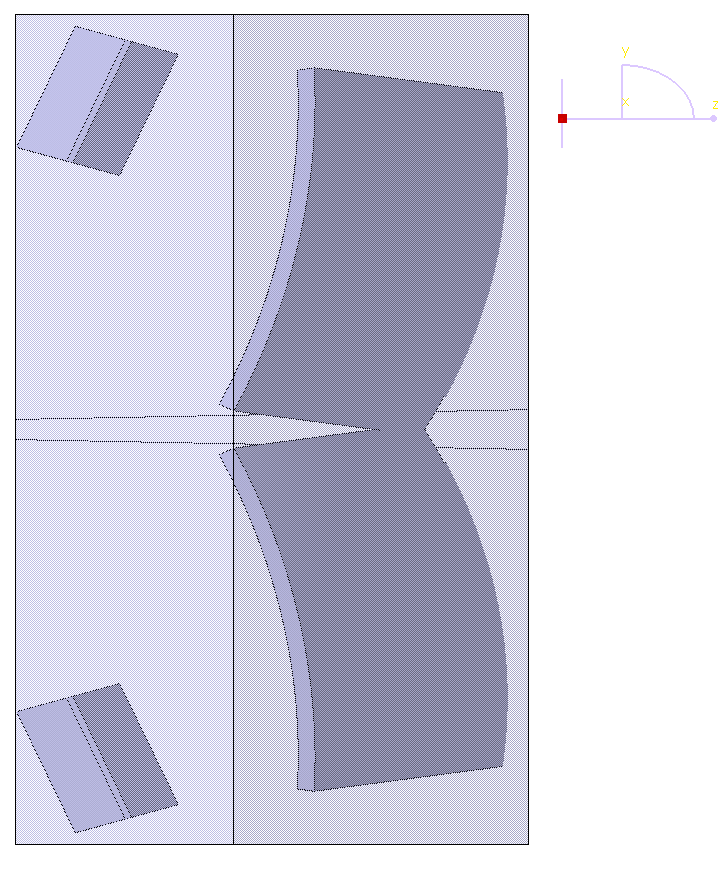
\includegraphics[width=1.0\textwidth]{pictures/RICH_MC_evolution_before.png}
\end{minipage}
\hspace{0.01\textwidth}
\begin{minipage}[b]{0.495\textwidth}
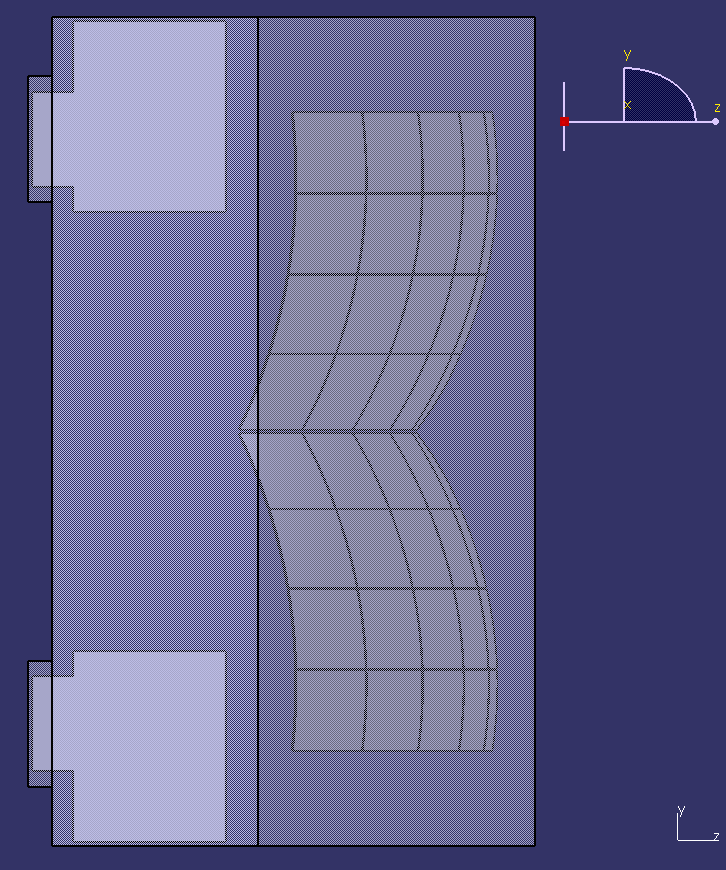
\includegraphics[width=1.0\textwidth]{pictures/RICH_MC_evolution_after.png}
\end{minipage}
\caption{Модель со старыми зеркалами (слева) и модель с новыми зеркалами (справа).}
\label{fig:MCgeoMirrorsEvolution}
\end{figure}

\begin{figure}[H]
\centering
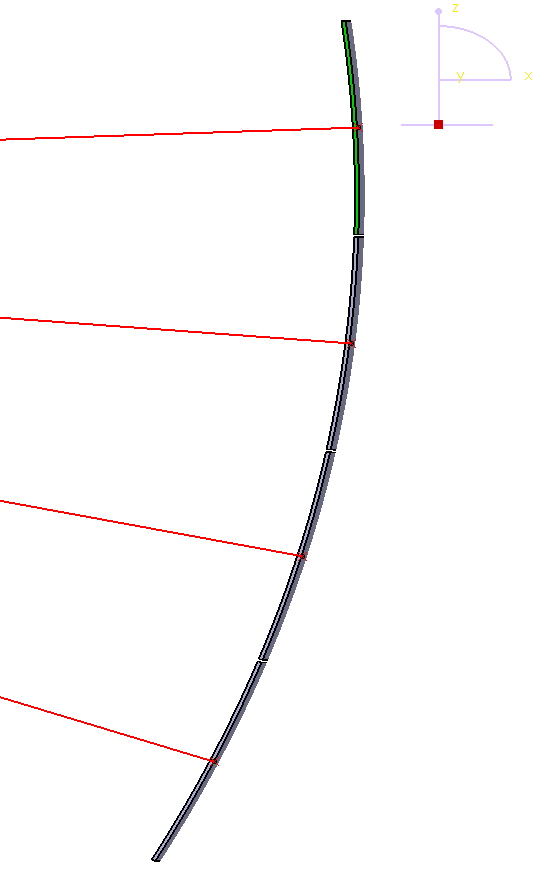
\includegraphics[width=0.3\textwidth]{pictures/Mirrors_4types_of_segments.png}
\caption{4 типоразмера сегментов зеркал, позволяющие собрать фокусирующую систему без зазоров.}
\label{fig:Mirrors4types}
\end{figure}

\subsection{Модель с ``малой рамой''.}

На раннем этапе была предложена конструкция опор зеркал, которая в дальнейшем была отвергнута из-за слишком большого количества материала в аксептансе. На \figref{fig:SmallFrameCADandMC} показана модель опор зеркал в САПР (слева) и в CbmRoot (справа).

\begin{figure}[H]
\begin{minipage}[b]{0.495\textwidth}
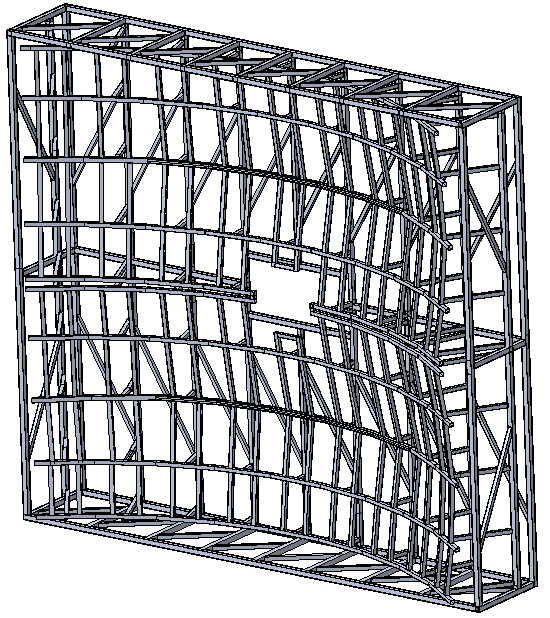
\includegraphics[width=1.0\textwidth]{pictures/Frame_small_CAD.png}
\end{minipage}
\hspace{0.01\textwidth}
\begin{minipage}[b]{0.495\textwidth}
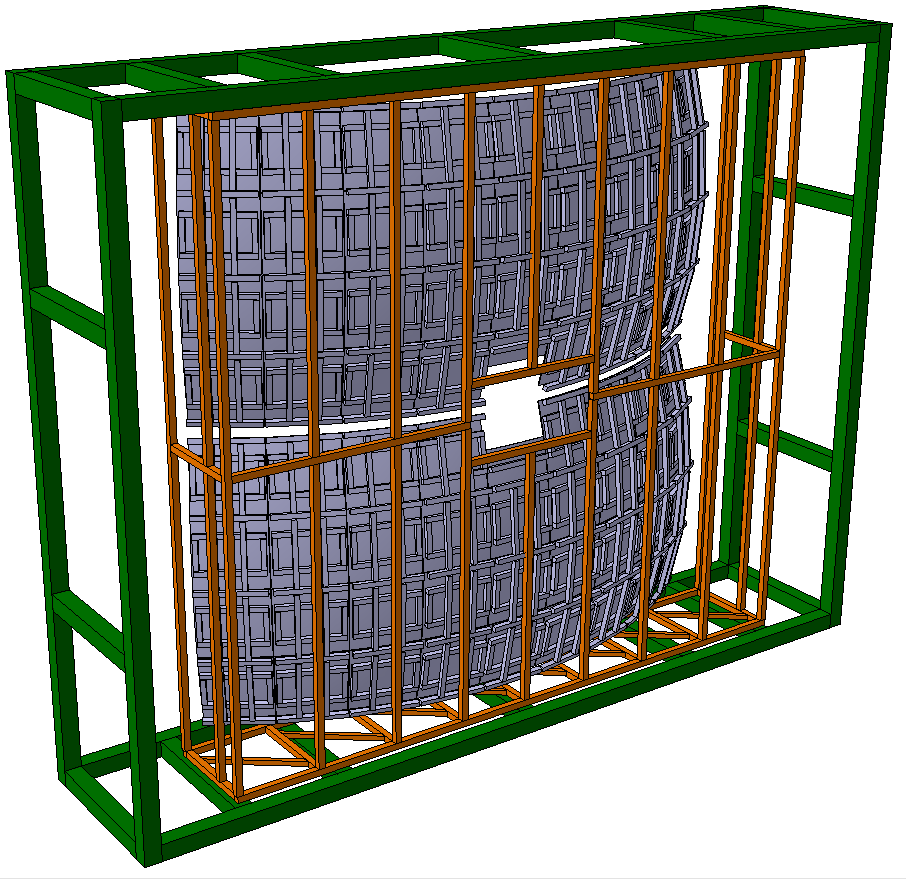
\includegraphics[width=1.0\textwidth]{pictures/Frame_small_MC2.png}
\end{minipage}
\caption{Ранняя модель опор зеркал в САПР CATIA~V5 (слева) и в CbmRoot (справа).}
\label{fig:SmallFrameCADandMC}
\end{figure}
